%
% 3_Arrokoth.tex
%
% (c) 2020 Prof Dr Andreas Müller, Hochschule Rapperswil
%
% !TEX root = ../../buch.tex
% !TEX encoding = UTF-8
%
\section{Arrokoth
\label{planet:section:arrokoth}}
\rhead{Arrokoth}

Arrokoth in \cref{planet:fig:arrokoth} ersichtlich, ist ein kleiner Asteroid aus dem Kuipergürtel, auch unter der ursprünglichen Bezeichnung (486958) 2014 MU69 sowie unter seinem Spitznamen Ultima Thule bekannt ist.
Der Name Arrokoth ist Powhatan/Algonquianisch und heisst „Himmel“.

Arrokoth ist das am weitesten entfernte Objekt, das jemals mit einer Raumsonde erforscht wurde.
Es wurde mit Hilfe des Hubble Weltraum Teleskopes 2014 vom New Horizions Wissenschaftsteam entdeckt.
Die Informationen zu Arrokoth sind von \cite{planet:arrokoth} entnommen.

Solche Weltraumschneemänner können nur entstehen wenn die eigene Gravitation kleiner ist als die starren Kräfte des Körpers.
Das bedeutet die Himmelskörper sind kleinere Objekte im Vergleich zu Planeten.
Zusätzlich dazu dürfen die einzelnen Asteroiden nicht mit grosser Kraft aufeinander treffen, das bedeutet verbinden der zwei Körper geschieht relativ langsam.
Wenn zwei Asteroiden mit grosser Geschwindigkeit aufeinander treffen, würden sie in kleinere Trümmer zerschmettert die über längeren Zeitraum wieder ein Asteroid bilden der widerum eine Kugelform hat.

\begin{figure}[h]
    \centering
    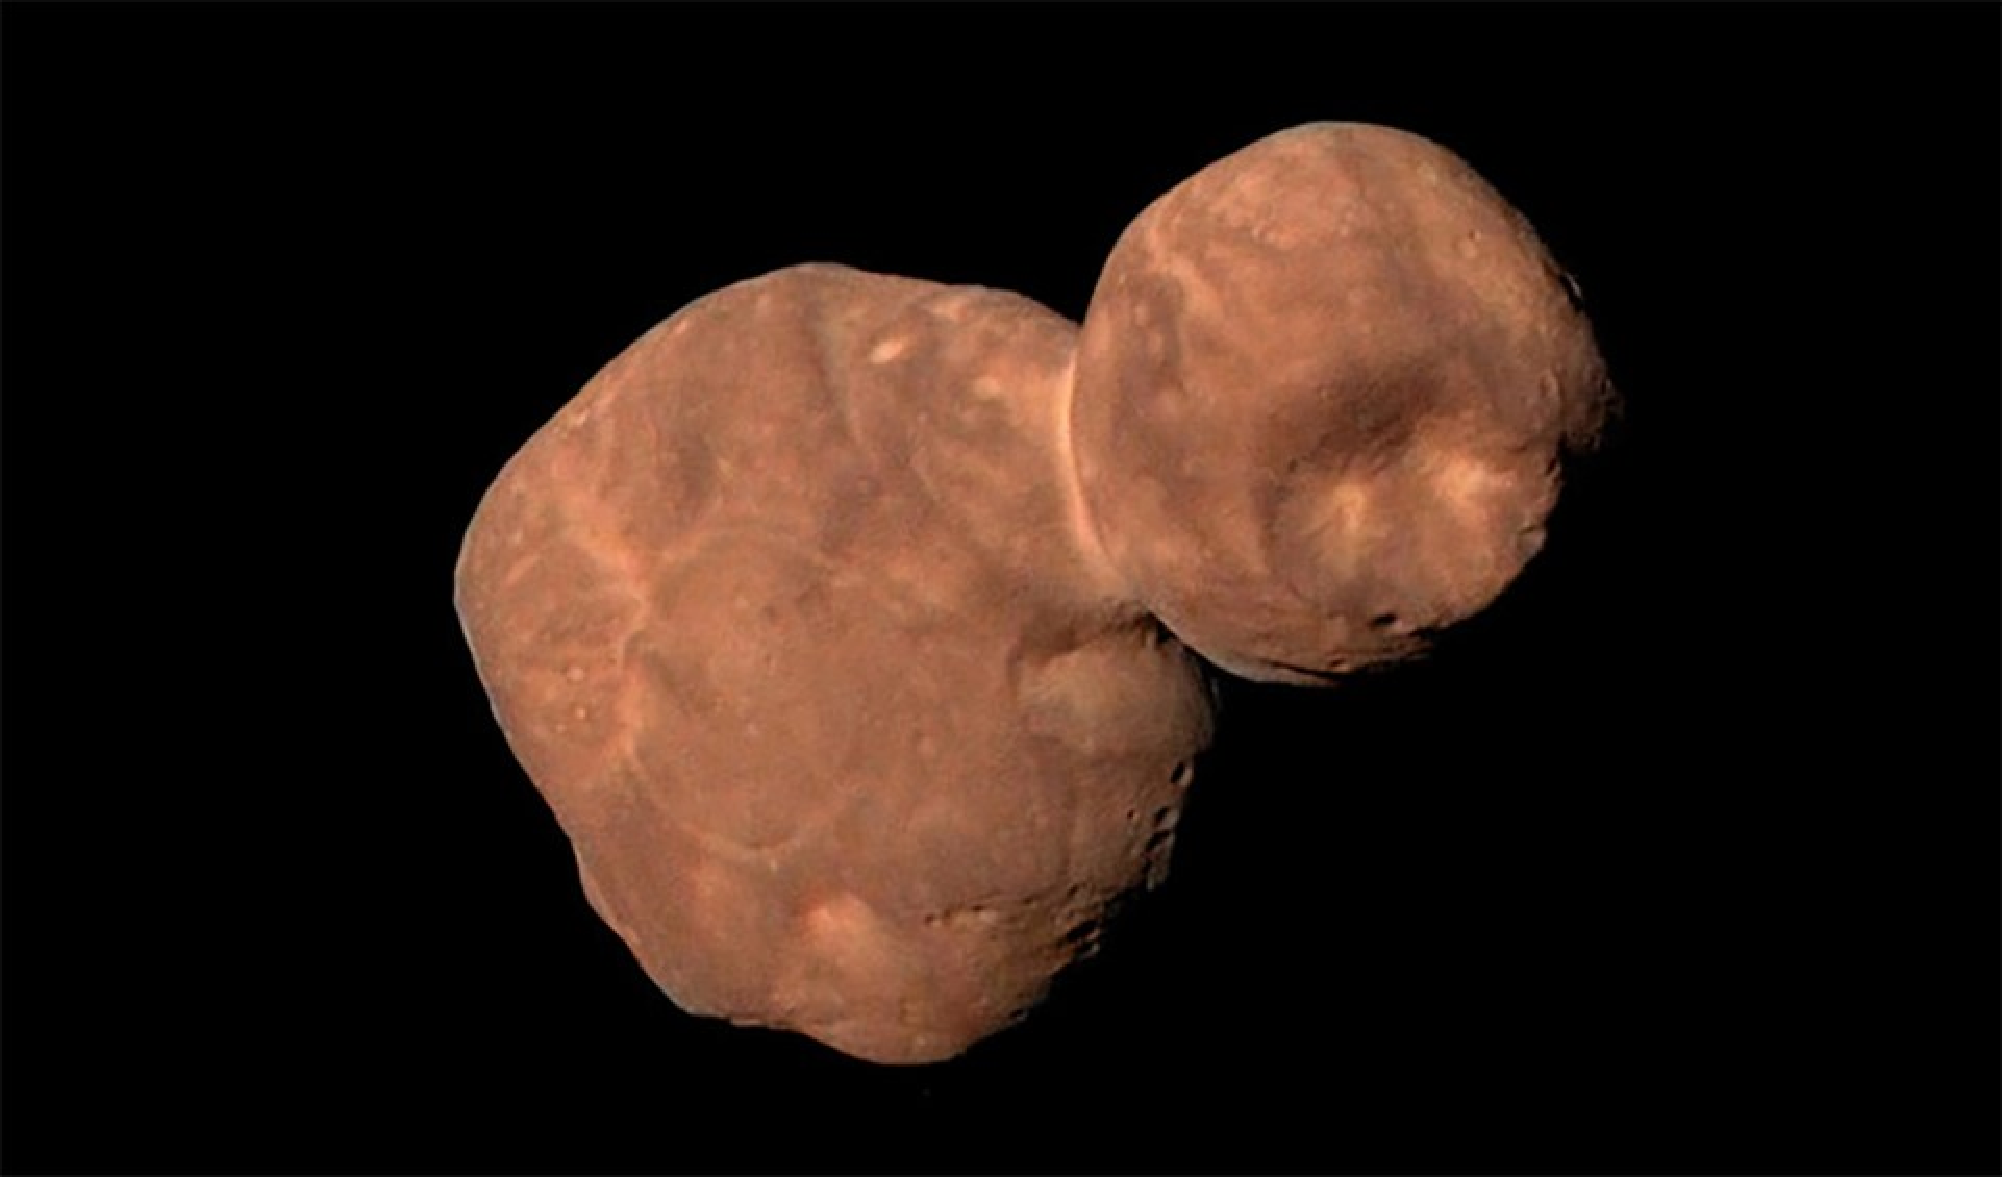
\includegraphics[width=\linewidth]{papers/planet/pictures/Arrokoth.pdf}
    \caption{Arrokoth aus dem Kuipergürtel \cite{planet:arrokothpic}
        \label{planet:fig:arrokoth}}
\end{figure}